\chapter{Implementierung}

\section{Einleitung}

Ziel dieser Arbeit war es, eine Simulationsumgebung für Sensorknoten zu schaffen. Es sollte viele verschiedene Arten von Sensorknoten geben, die jeweils einen oder mehrere verschiedene Sensoren besitzen. Mit diesen Knoten sollte ein Netzwerk aufgebaut werden, um die Umgebungsparameter eines Gebietes zu erfassen.
Die Daten der Simulation sollten visualisiert und ausgewertet werden.

\section{Aufbau und Struktur}

\subsection{Klassenübersicht}

Die Klassenübersichten wurden teilweise mit Hilfe von doxygen\cite{doxygen} erstellt. 

\begin{center}
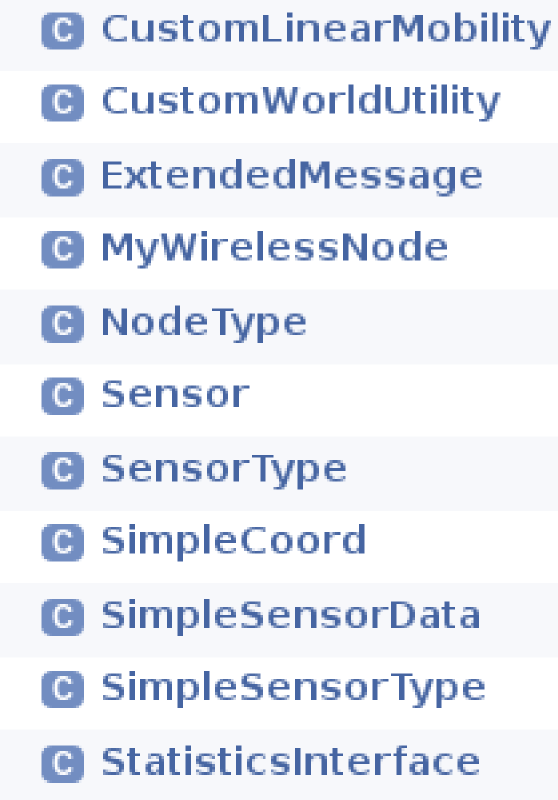
\includegraphics{Klassenuebersicht}
\end{center}

\paragraph{CustomLinearMobility}

\begin{center}
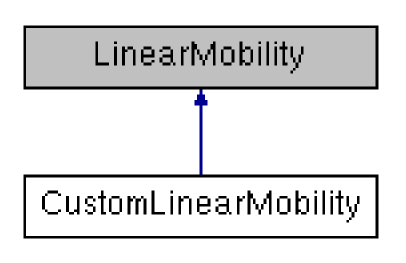
\includegraphics{CustomLinearMobility}
\end{center}

Diese Klasse erbt direkt von der in MiXiM definierten LinearMobility. Sie ist um einige Parameter erweitert, die es ermöglichen, dass die Knoten beschleunigen können und eine maximale Geschwindigkeit \textbf{maxSpeed} erreichen, sollte eine definiert sein.
Der Parameter \textbf{maxSpeed} kann ebenso auf 0 gesetzt werden, um die Knoten von mobil in stationär umzuwandeln.

\paragraph{CustomWorldUtility}

Die Klasse CustomWorldUtility ist eine der wichtigsten für die Simulation. Sie repräsentiert den \textbf{Playground}, also den Bereich indem sich die Knoten befinden. Sie erbt von der Klasse BaseWorldUtility aus dem MiXiM-Framework. BaseWorldUtility stellt die nötigen Funktionalitäten für den Playground bereit. \newline

\begin{center}
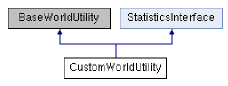
\includegraphics{CustomWorldUtility1}
\end{center}

Zusätzlich dazu stellt die Klasse selbst die notwendigen Parameter für die Umwelt bereit. Nach dem Starten der Simulation steht darin jeweils ein zweidimensionales Array pro Sensortyp bereit: temperatureArray, pressureArray, humidityArray und lightArray. Diese enthalten die Parameter der Umgebung; temperatureArray beinhaltet zum Beispiel, wie der Name schon sagt, Informationen über die Temperatur. \newline
Es kann zu Beginn der Simulation entschieden werden, ob neue Werte berechnet werden sollen oder die bereits vorhandenen Werte für die Umgebung übernommen werden sollen. Die Arrays besitzen die gleiche Größe wie der Playground. Diese Größe ist auch zusätzlich in den Parametern sizeX und sizeY gespeichert.

\begin{center}
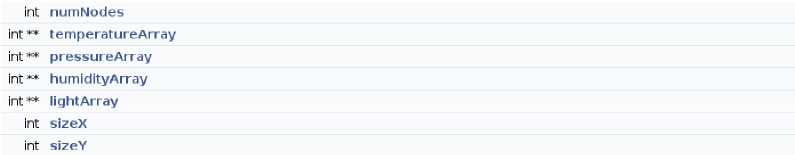
\includegraphics[width=\textwidth]{CustomWorldUtility3}
\end{center}

Zum Erstellen neuer Daten kann die Funktion \textbf{generateEnvironmentData()} genutzt werden. Es ist dadurch auch möglich während der Simulation neue Werte zu generieren, indem man diese Funktion aufruft. Die Funktion legt pro Umweltparameter eine xml-Datei im Ordner \textit{WorldModel/data} an. Jede der xml-Dateien wird beim Start mit Hilfe der Funktion \textbf{readXML(int)} eingelesen, verarbeitet, also in ein Array umgewandelt und anschließend in der Klasse gespeichert. \newline
Sollte nun ein Sensor nach dem Wert an seiner aktuellen Position fragen, so kann diese Klasse mit Hilfe der Funktionen \textbf{generateMessage(const char*)} und \textbf{sendSensorResponse(std::string, cGate *)} eine Antwort generieren. Die Position kann dabei mit der Klasse \textbf{SimpleCoord} und der Wert an dieser Position mit \textbf{SimpleSensorData} repräsentiert und per Nachricht verschickt werden.

\begin{center}
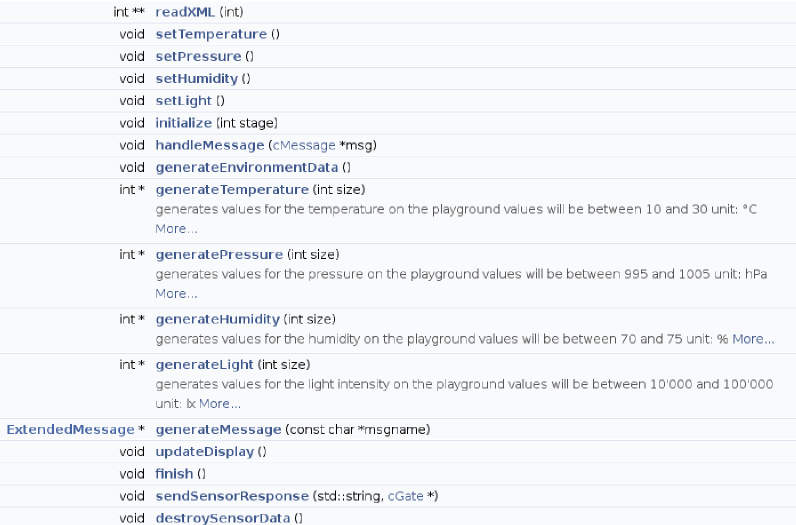
\includegraphics[width=\textwidth]{CustomWorldUtility2}
\end{center}

\subsection{Netzwerk}

alle elemente in NED beschreiben (also alles was nicht schon in der vorherigen section erklärt wurde)

\section{Funktionsweise}

was funktioniert wie
was wurde überhaupt umgesetzt
was fehlt evtl/verbesserungsideen